\chapter{Methods}\label{chapter:method}

{ \color{red}

    about 10-30 pages (rather more I guess)

    \begin{itemize}
        \item (1/3 of thesis)
        \item start with a theoretical approach, describe the developed system/algorithm/method from a high-level point of view,
        \item go ahead in presenting your developments in more detail
        \item make sure to not refer to results section too much. rather leave info out if it cannot explained well without looking at the results
    \end{itemize}
}


\section{Causal Model}
For the exact comparison of importance between the model and its explanation it is imperative to know the ground truth of the training data. A structural causal model (SCM) can define variables and the independent mechanisms with which they interact precisely. We want to define an SCM that closely mirrors image generation processes as they happen in realistic scenarios. 
Explicitly using a generating SCM has previously been done to test new attribution methods \cite{Parafita2019, Wilming2023, Goyal2019, Reimers2019, Reimers2020}. A few other works evaluating XAI methods with a known ground truth have implicitly used structures akin to an SCM without defining it in causal language \cite{Kim2018, Yang2019}. 

The causal graph and its entailed distribution used for our experiment are defined as follows: 
\begin{align*}
    & G := \mathcal{N}(0.5,0.02) \\
    & N_w := \mathcal{N}(0.5,0.02) \\
    & N_s := \mathcal{N}(0.5,0.02) \\
    & W := \rho * G + (1-\rho)* N_w \\
    & S := \rho * G + (1-\rho)* N_s \\
    & \mathcal{X} = f_{image}(W, S, Z) + N_{x} \\
\end{align*}

\begin{figure}[H]
    \centering
    \includegraphics[width=0.9\textwidth]{pics/generating_scm.png}
    \caption{Structural causal model for first experiment.
        In the top right corner the distribution of the variables Watermark $W$ and Shape $S$ are plotted against each other to show the effect of changing $\rho$ (here $\rho = 0.6$)}
    \label{fig:generating_scm}
\end{figure}

The SCM as seen in \autoref{fig:generating_scm} serves as a starting point for our first experiment. It is an additive model using Gaussian distributions for the noise terms.  The meta-variable \textit{spurious-to-core ratio} $\rho$ adjusts how much information is shared between the true class information (shape), which we name \textit{core feature} following \cite{Singla2022} and the watermark or \textit{spurious feature} through a shared common ancestor named generator $g$. Ratio $\rho$ is a hyperparameter of our image generation process in a similar sense to how hyperparameters are defined in Karimi et al. \cite{Karimi2023}. While \cref{fig:generating_scm} depicts the generating model of the training dataset, \cref{fig:egp} shows how this is embedded into the mechanic process of generating explanations. 

\begin{figure}
    \centering
    \includegraphics[width=0.9\textwidth]{thesis_latex_template/pics/explanation_generation.png}
    \caption{Explanation generating process}\label{fig:egp}
\end{figure}

The idea of investigating the effect of such a coupling ratio $\rho$ was inspired by Wilming et al. \cite{Wilming2023}, who also used a \textit{signal-to-noise} ratio in their generating model. Instead of a confounding model their learned data instances are colliders of their label and a suppressor variable. The expected explanation importance of this suppressor feature therefore ought to be zero, as long as the collider is not intervened on. 

A second parameter which we keep fixed for our experiment, determines how prevalent the spurious feature is in the data. We set this parameter which could be termed \textit{prevalence} to 0.5, so that just as many images have a watermark as not. It is important to note that this particular SCM is just one of many possible ways to model how spurious features might interact with core features. It attempts to follow the logic of how images are generated or selected in real datasets. Here, it particularly looks at pathways for the generation of \textit{Clever-Hans} or \textit{watermark} features, often present in image datasets \cite{Lapuschkin2019}. As visible in \cref{fig:equivalent_scm} different causal models can produce an equivalent distribution of the two latent factors in question (watermark and shape). One can think of many more variations of SCMs which are able to produce the same correlation, so the choice of using the confounder version as in \cref{fig:generating_scm} is mainly due to its ease of implementation. Another consideration is that the interpretation of $\rho$ as a coupling ratio between the core and spurious feature helps in understanding its supposed effect on the prediction and explanation. The motivation for that is also to investigate the strength of coupling necessary for the spurious feature to become important. 

The direction of causal links for images is highly debatable and shall not be the focus of this work. Whether the selection of the AI researcher reducing costs with free images resulted in classes being polluted with watermarks (\cref{fig:equivalent_scm}\textbf{a}), or whether a scientist marked x-rays with their diagnosis (\cref{fig:equivalent_scm}\textbf{b}) is indistinguishable for AI models. 
Instead, we only want to find to what degree a neural network learns, and attribution method explains the distribution generated by a particular SCM.

To evaluate the results of the current experiment and see how having a different SCM might influence the outcome we will later look at other generating SCMs too (\cref{chapter:results}).

\begin{figure}[H]
    \centering
    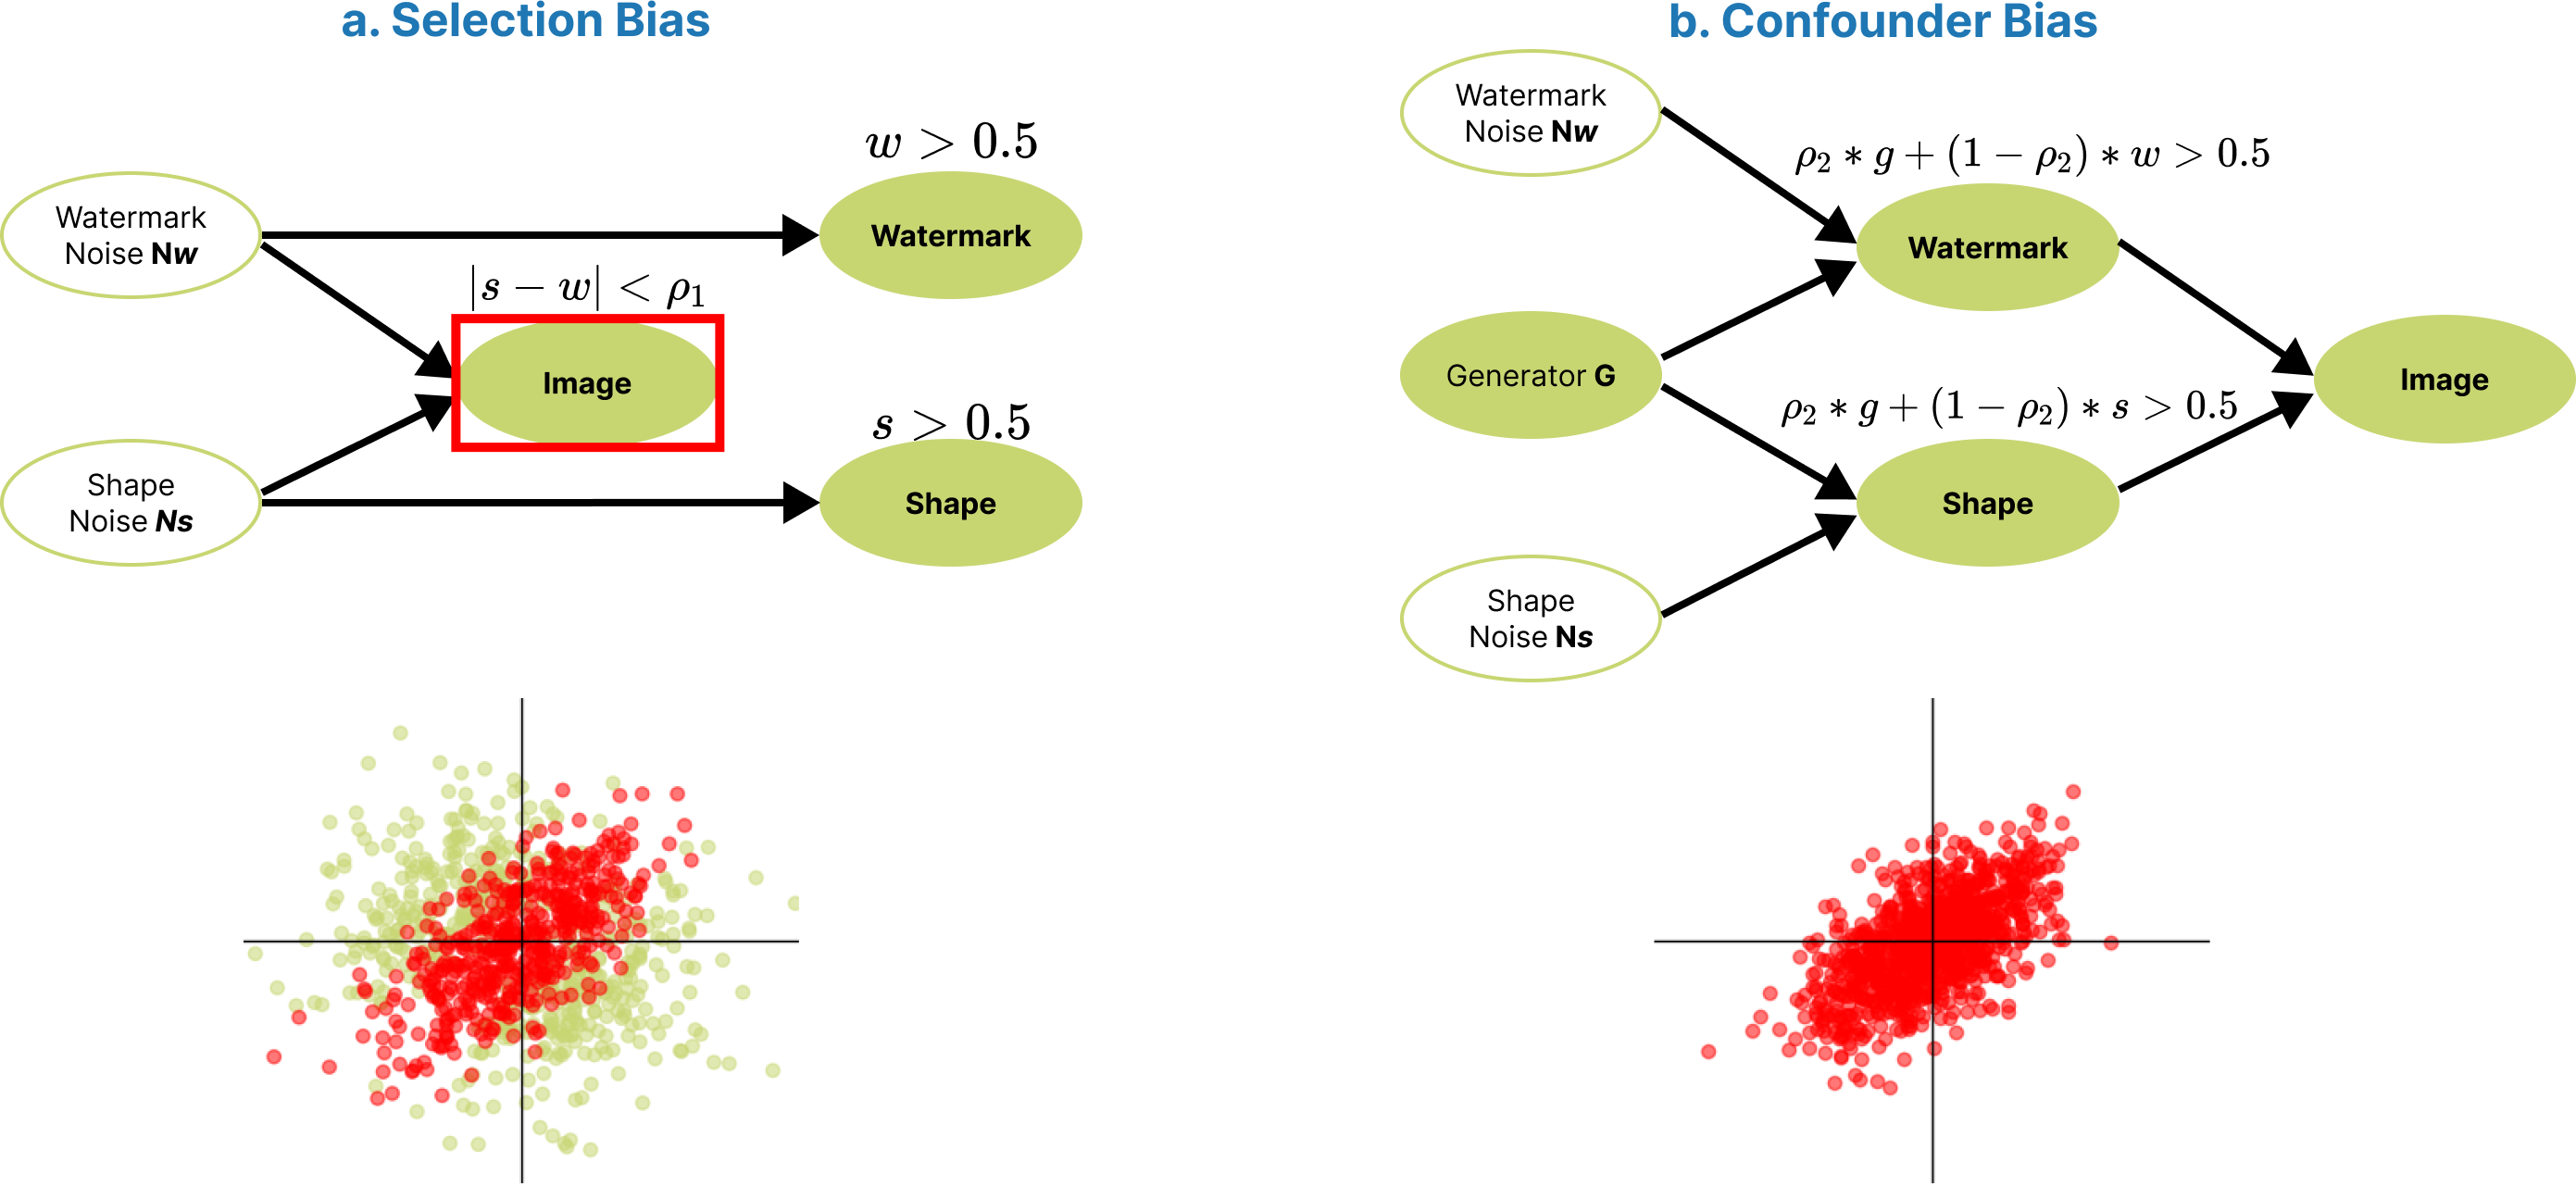
\includegraphics[width=0.8\textwidth]{pics/equivalent_scm.png}
    \caption{SCMs typically found in image datasets.
    \textbf{a.} Selection Bias \textit{(researcher chooses images from free online collection with watermarks)}
    \textbf{b.} Confounder Bias \textit{(e.g. scientist marks positive x-ray scans with sign)}}
    \label{fig:equivalent_scm}
\end{figure}

\begin{figure}[H]
    \centering
    \tikzset{%
        neuron/.style={
                circle,
                draw,
                minimum size=8mm
            }
    }
    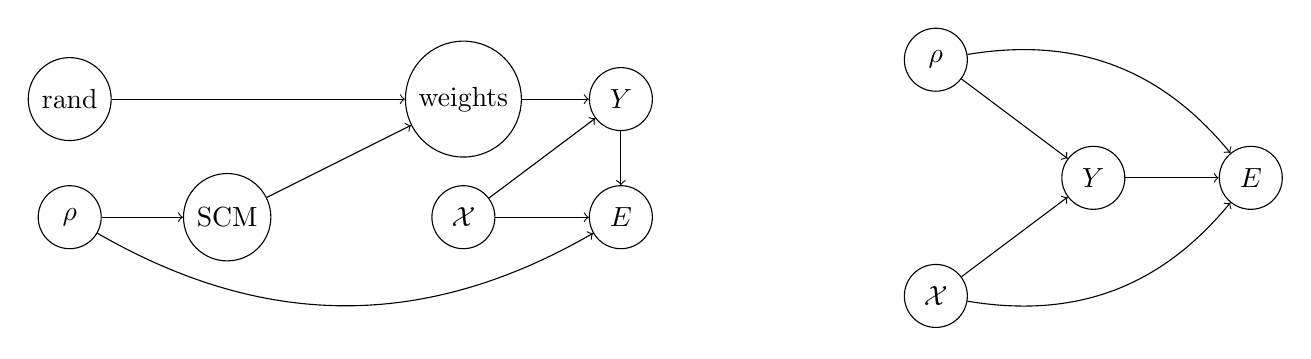
\begin{tikzpicture}[every node/.style={ draw, minimum size=8mm, align=center},]

    % generating model:
        \node [neuron]  (r) at (0.0,1) {$\rho$};
        \node [neuron]  (rs) at (0,2.5) {rand};
        \node [neuron]  (scm) at (2,1) {SCM};
        \node [neuron]  (ws) at (5,2.5) {weights};
        \node [neuron]  (x) at (5,1) {$\mathcal{X}$};
        \node [neuron]  (p) at (7,2.5) {$Y$};
        \node [neuron]  (e) at (7,1) {$E$};

        \draw[->] (r) -- (scm);
        \draw[->] (rs) -- (ws);
        \draw[->] (scm) to (ws);
        \draw[->] (ws) -- (p);
        \draw[->] (x) -- (p);
        \draw[->] (x) -- (e);
        \draw[->] (p) -- (e);
        \draw[->, bend right=30] (r) to (e);
        
    % simplified causal model:
        \node [neuron]  (r) at (11,3) {$\rho$};
        \node [neuron]  (x) at (11,0) {$\mathcal{X}$};
        \node [neuron]  (p) at (13,1.5) {$Y$};
        \node [neuron]  (e) at (15,1.5) {$E$};

        \draw[->] (r) -- (p);
        \draw[->] (x) -- (p);
        \draw[->, bend right=30] (x) to (e);
        \draw[->] (p) -- (e);
        \draw[->, bend left=30] (r) to (e);
    \end{tikzpicture}
    \caption{Explanation Generation Process (left), Simplified Causal Process (right)}
    \label{fig:test_tikz}
\end{figure}

\subsection{Watermark Benchmark Dataset W-dSprites}\label{section:causal_model}
Although this thesis is not the first work to use a toy dataset with known generating factors to evaluate attribution methods, we aim to find data which is as simple as possible and yet mirrors the main workings of a realistic computer vision problem.  For this we adapted the dSprites dataset \cite{dsprites17} by adding small watermarks in the shape of '\textit{w}'s to some images. The dSprites dataset was originally constructed as a means for testing the degree of disentanglement a machine learning model has achieved. It contains images with rectangles, ellipses or hearts in varying positions, scales and rotations. To simplify the task even more we only use the rectangle and ellipse class for our experiment. Another motive is that in a binary classification task positive and negative relevance might be used in varying strategies for prediction. In theory this could make the class-insensitivity studied by Sixt et al. \cite{Sixt2020} visible or counteract it. Further details can be found in the appendix \cref{appendix:dsprites}.

\begin{figure}[H]
    \centering
    \includegraphics[width=0.6\textwidth]{pics/dsprites_examples.png}
    \caption{First row: images from the original dSprites dataset, second row: images from the watermarked dataset W-dSprites with small \textit{w} as a watermark on some images and Gaussian noise added.}
    \label{fig:dsprites_examples}
\end{figure}

\section{Generating Explanations with Concept Relevance Propagation}
Producing explanations using concept relevance propagation requires decisions on the backpropagation rule(s), on the conditioning sets and potentially further hyperparameters. 
We follow the recommendations or default settings of CRP's authors \cite{Achtibat2022, Achtibat2023} and best practices \cite{Kohlbrenner2020} as closely as possible .
For the backpropagation we apply the $LRP_{\varepsilon -z^+- b^-}$ - rule as recommended by \cite{Kohlbrenner2020}. Due to the simplicity of our CNN model no more model canonization steps need to be applied. See \cref{appendix:lrprules} for further technical details. 

In principle, neurons in every layer of a model can be conditioned on using the CRP-approach. However, the resulting attribution maps are not necessarily producing disentangled but abstract enough concepts. When looking at a \textit{concept-conditional} attribution maps from the earlier layers, one will likely see low-level features. In the later linear layers before the output the potentially disentangled concepts might get mixed together again for the final decision. According to \cite{Dreyer2023a, Zeiler2013} the last convolutional layer is ``most likely representing disentangled representation''. Our trials investigated both the last convolutional and the first linear layer of the simple cnn-model. It is not entirely clear whether the extremely small size of our model hinders a comparison to realistic scenarios, but training significantly larger models would have been too computationally expensive for this experiment. 


\begin{itemize}
    \item how do fraunhofer people do it in their paper? what are their recommendations?
    \item each different score/ heatmap / reference set etc. that can be (and should be for this case?) computed
    \item as recommended by fraunhofer people: always use class-specific conditional relevance
    \item should I keep class the same or change per instance?
    \item it would be best, to test multiple of the proposed methods for concept specific attribution: Not just the pure heatmaps but also the relevance maximization sets and their receptive field information
    \item Since the models in our experiment do not have special skip connections or recurrence we can expect the complete relevance to go through the set of neurons of one layer. 
\end{itemize}

\section{Data Ground Truth Correlation $m_0$}
Measure $m_0 = \rho$ could be just pure correlation between 2 values of shape and watermark. but through causal model might be a bit inaccurate or not describing exactly what the data distribution is like. Therefore something like mutual information might be a better measure...
Compare why what is better, but probably plot pure $\rho$ in plots anyway (plus maybe others)

\begin{figure}
    \centering
    \includegraphics[width=0.5\textwidth]{thesis_latex_template/pics/test.png}
    \caption{$\rho$ plotted against other possible ways to measure ground truth data importance/ correlation of $w$ and $s$}
    \label{fig:finding_rho}
\end{figure}

\section{Establishing a Ground-Truth Model Feature Importance $m_1$}\label{section:gt_measure}
In contrast to realistic application scenarios our causal dataset enables us to establish the ground truth importance of features for a trained model. Similar to recent work on causal attribution \todo{cite} the causal effect of an intervention upstream on the output of a model can be measured in the following:
\begin{center}
Average Causal Effect of latent factor $W$ on output $Y$ \\
\begin{equation}
\displaystyle ACE = \mathbb{E} [ Y \ | \ do(W=1) ] - \mathbb{E} [ Y \ | \ do(W=0) ] 
\end{equation}
\end{center}
The intervention on a given latent factor is straight-forward, as our factors of interest are both binary variables (watermark and shape). Due to our knowledge of the ground truth we can just feed one image with the watermark and the same image without it through the neural network. Thereby achieving a perfect intervention on our latent factor.  
However it is not naturally clear how to define the output of a model. One can either measure the average causal effect on the output layers' logits, which change in a continuous fashion, or the effect on the binary prediction. In our example this would be equivalent to the percentage of images for which the prediction flips, when the factor is flipped. 

\subsection{Mean Logit Change}
\begin{itemize}
    \item it is basically the causal effect of intervening on a latent factor on the models output
    \item theoretically the intervention must have exactly the same causal effect on the explanation as on the mean logit change???
    \item is most accurate, as it also reflects small changes in the logits, that do not flip the prediction
    \item for intermediate values of $\rho$ like $0.65$ one could expect the models to have learned some importance of the watermark, which slightly reduces/strengthens the confidence, but does not flip over the prediction
    \item it might still be interesting to see this slight effect. As in the \textit{worst case} out-of-distribution prediction, this effect might take over, over the shape features effect. 
\end{itemize}
For the W-dSprites binary classification task, the output layer consists of 2 values $y_0$ and $y_1$. The network predicts \textit{rectangle} when $y_0 > y_1$ and \textit{ellipse} otherwise. To compute the mean logit change when intervening on our watermark spurious feature $x$, we take a sufficient amount of samples $\mathcal{X}$ from our dataset and feed them through the model. When $W=1$ the images additionally contain a watermark, when $W=0$ not. 

The Mean Logit Change is computed the following way:

% euclidean distance (=earth mover distance), absolute difference, should it be averaged over logits, kernel (like Karimi)
\begin{equation}
\displaystyle 
MLC =\frac{1}{|\mathcal{X}|} \sum_{c \in \mathcal{X}} \frac{|\vec{y}_{\mathrm{x}, W=1}- \vec{y}_{\mathrm{x}, W=0} |}{|\vec{y}|}
\end{equation}

\subsection{Prediction Flip}
Computing the Prediction Flip follows mostly the same approach as the mean logit change. The only difference is that instead of computing the average effect of the continuous multivariate output vector $\vec{y}$ we consider the prediction to be the binary class variable $y$ which is 0 for rectangle and 1 for ellipse predictions. 

We expect this variant of the prediction variable to be less sensitive to the spurious watermark feature $W$. The reason being, that while the continuous output (i.e. \textit{confidence}) might already be affected by the spurious feature for weaker biases, the prediction will only flip once the spurious feature becomes more important. 

\begin{equation}
\displaystyle 
PF =\frac{1}{|\mathcal{X}|} \sum_{\mathrm{x} \in \mathcal{X}} |y_{\mathrm{x}, W=1} - y_{\mathrm{x}, W=0} |
\end{equation}

\section{CRP Explanation Importance $m_2$}\label{section:measure}
Our goal is to compare the causal effect of an upstream intervention on the true feature importance and the explained feature importance. After having defined how to measure the models true feature importance, we need to repeat the process for the explanation produced by CRP. It is not well known how humans perceive changes in an explanation and there is no agreed upon scale of importance, so we believe it is best to construct multiple measures to test against each other. Most of the proposed metrics are derived from existing work on evaluating feature importance in XAI \cite{Arras2022} \\

Each candidate should be a variation of measuring the effect of intervening on $x$ on the explanation:
\begin{center}
Average Causal Effect of latent factor $x$ on explanation $\mathfrak{e}$: \\
\begin{equation}
\displaystyle ACE = \mathbb{E} [\mathfrak{e} \ | \ do(w=1) ] - \mathbb{E} [ \mathfrak{e} \ | \ do(w=0) ]
\end{equation}
\end{center}
The core question is, how much of the influence on the explanation of changing $\rho$ goes through our prediction. This is one way to describe the fidelity of the explanation with the model. The proposed measures however incorporate other notions of goodness applied for XAI such as \textit{intelligibility, complexity} and \textit{ user-friendliness}. \\

The measures introduced in the following are roughly ordered from measures being most true to the numerical effect to measure closest to importance changes perceivable by humans. This ordering also orders them based on their complexity. While the first measure requires the user to compare multiple heatmaps pixel-wise, later metrics use only one pixel or a reduced (hopefully human-understandable) concept. 

{\color{gray}
What about causal effect of changing the class, while keeping the watermark on? (should diminish when bias stronger)
\begin{equation}\displaystyle
    \mathbb{E} [RMA \ | \ do(S=1), W = 1  ] - \mathbb{E} [ \mathfrak{e} \ | \ do(S=0), W = 1 ]
\end{equation}
}

\subsection{Relevant Attribution Change}
An intuitive way to calculate explanation importance for neurons in a layer using CRP is to measure the average causal effect of an intervention on the attributions directly. This approach tries to emulate the \textit{mean logit change} of the prediction for the concept-based explanation. In a given layer $\ell \in L$, computing conditional attributions for each of the $|\ell|$ neurons results in $|\ell|$ concept-conditional heatmaps. Also, the total relevance of those neurons for the overall prediction can be computed using CRP.
The causal effect of intervening on the spurious watermark feature on one neuron is then the (absolute?) difference between its attribution map of one image with a watermark and the same image without a watermark. For an approximation of the total difference for a model, we weigh each neurons attribution map difference with the neurons relevance for the prediction. 
Many related works remove negative relevances in attribution maps to enable comparison with purely positive methods and avoid cancelling-out effects. We believe however, that a spurious feature can be equally negatively as positively attributed, for a model to be biased. Therefore we experiment with taking the absolute difference of heatmaps instead of zeroing out negative relevance. 
Other potential ways to aggregate over differences is to apply the method of \cite{Karimi2023} using kernels or cosine similarity as in \cite{Dreyer2023a}. The latter however disregards potential sign-flip of a pixel as significant. 

Extend on why using 10 models with different seeds and K different images (that are well distributed?) is enough to compute measure? 
\begin{align*}
& R_i^{\ell}(\mathrm{x}) = R(\mathrm{x} | \theta=\{i, y\}) \\
& r_i(\mathrm{x}) = R(i | \theta=\{y\}) \\
& RAC = \frac{1}{|\mathcal{X}| }\sum_{\mathrm{x} \in \mathcal{X}} \sum_{i \in \ell} || r_i(\mathrm{x}_{(W=1)}) * R_i(\mathrm{x}_{(W=1)}) -  r_i(\mathrm{x}_{(W=0)}) * R_i(\mathrm{x}_{(W=0)})  || \\
& RAC_{\rho} = \frac{1}{|M_\rho|}\sum_{m}^{M_{\rho}} RAC(m)
\end{align*}

While this weighted difference is constructed to measure the causal effect of intervention on the explanation as closely as possible, it ignores the core idea of CRP's potential usefulness. If adding or removing a watermark has a significant effect on some background pixels far away from it, this is not in line with desirable properties of a good explanation such as interpretability or even fidelity to the ground truth importance. It is likely that through the coupling of watermark and shape in our experiment, the changes of relevance do not only affect the watermark region itself but at least the shapes importance too. 
Another potential downfall for human intuition is the way more localized concepts are attributed in comparison to more global or wide-spread concepts. Achtibat et al. \cite{Achtibat2022} show an example where the eye of a dog wrongly seems to be more important than its fur in a general attribution map, because it is concentrated on a smaller region. A similar thing can potentially happen with our experiments watermark, as it fills a small region in comparison to the larger shape feature. 

Arguably, this method covers the information-theoretic difference when intervening on $W$ most completely. However...

\subsection{Importance in Ground-Truth Region}
In \cite{Arras2022} two metrics for the analysis of importance in pixel maps are introduced. Relevance Mass Accuracy (RMA) measures the ratio of relevance within a bounding box around a feature to the total relevance. Relevance Rank Accuracy (RRA) rates the percentage of pixels in such a bounding box that fall within the $k$ most important pixels in the heatmap.

\subsubsection{Relevance Mass Accuracy (RMA)}
Bau et al. \cite{Bau2017, Bau2020} have defined a similar measure to compare an explanation importance to a ground truth, which they term IoU (from \textit{Intersection over Union}). Both these works assume the perfect attribution of importance to one feature to be a binary mask, which is 1 inside and 0 outside the features region. \\

For our localized metric we apply a strategy resembling their evaluation score. 
Luckily, the authors of CRP have already defined \textit{local concept importance}, evaluating the conditional attribution to a concept in a predefined region. 
While RMA in the Clevr-XAI benchmark uses the exact pixel-boundary of an object, we use a bounding box around the watermark \textit{w}. This is not only due to simplicity but also because the small model we apply smoothes out relevance over a region because of max-pooling. \\

The \textit{localized relevance score} is the ratio of conditional relevance attributed to a certain region of an image. In our case, the region of interest are pixels in the bounding box $B$ around the watermark. 
\begin{align*}
\displaystyle
& R_B(\mathrm{x}) = \sum_{p_x \in B} R_{p_x}(\mathrm{x} | \theta)\\
& R(\mathrm{x}) = \sum_{p_x \in x} R_{p_x}(\mathrm{x} | \theta) \\
& RMA(\mathrm{x}) = \frac{R_B(\mathrm{x})}{R(\mathrm{x})} \\
& RMAC =\frac{1}{|\ell| |\mathcal{X}|} \sum_{i \in \ell} \sum_{\mathrm{x} \in \mathcal{X}} |RMA(\mathrm{x}_{(W=1)}) - RMA(\mathrm{x}_{(W=0)})|
\end{align*}


\begin{itemize}
    \item good about it: humans look at the heatmaps and only see whether the watermark is colored or not to identify its importance.
    \item problem: humans have a hard time estimating the overall importance of concepts/features if they have varying spatial extend, see \cite{Achtibat2022} about noses and fur of dog
    \item maybe also note \cite{Sixt2022a}: Humans are not good at identifying biases by looking at heatmaps or concept heatmaps?
    \item argue that at least in our case we have non-overlapping importance between watermark and shape, so attribution maps might be at least a bit more applicable 
    \item so if watermark is even just a little bit red, it will be important to humans
    \item even bigger problem: NN do not disentangle concepts strictly. therefore the concepts found could always encode watermark and shape feature at the same time. this effect is strongly visible in our benchmark
    \item question: how much is the result explained by the spurious feature?
    \item will be taken as the baseline. all other more reduced methods can be benchmarked with this too ? 
\end{itemize}

\subsubsection{Relevance Rank Accuracy (RRA) or Pointing Game}
The second metric adapted from \cite{Arras2022} but also in similar ways introduced in other works is \textit{Relevance Rank Accuracy} or a related method nick-named \textit{Pointing Game}.  
Relevance Rank Accuracy orders the input features (i.e. pixels) by relevance and finds the $k$ most relevant pixels. The rank $k$ is equal to the size of the mask of the feature in question, here the bounding box around the watermark. Computing the ratio of the top-k relevant pixels inside of the bounding box $B$ to k yields the \textit{Relevance Rank Accuracy}:

\begin{align*}
& P_{top-k} = (p_1, p_2,...,p_k | |R_{p_1}| > |R_{p_2}| > ... > |R_{p_k}| ) \\
& \frac{|P_{top-k} \cap B|}{|B|}
\end{align*}
Due to the binary nature of our problem we want to account for negative relevance just as much as for positive relevance, hence we take the absolute relevance values.
Arguably, this metric loses even more information on whether at least some importance is assigned to the spurious feature (watermark). Previous work has pointed out many issues with this or similar methods. However it reduces the complexity of the explanation by only looking at the k-most important pixels. \\

A step towards even more reduced complexity is the \textit{Pointing Game} metric, first introduced in blub. The only difference between RRA and the Pointing Game metric is, that the latter \textit{binarizes} the question by setting $k$ to 1. If the most important pixel is inside the watermark bounding box $B$, the watermark is important, otherwise not. \\

We expect these two methods to not assign high importance to the watermark feature, because it has a relatively small region and is for most values of $\rho$ only expected to be the \textit{second}-most important feature. In this regard, they most probably closer follow the ground-truth importance of the \textit{prediction flip} metric.

\subsection{Interpretation Techniques from CRP Work}
The authors of CRP embed the approach into a multitude of potential concept-based interpretation techniques. Their motivation is to gain more abstract, reduced explanations, while still potentially using multiple concepts. The underlying assumption is that the neurons in layers of deep neural networks encode human-understandable concepts hierarchically from low-level to abstract \cite{Zeiler2013,Bau2017}. Although this assumption seems to work mostly for large and deep CNN and complex, realistic image datasets, the general idea can be applied in our experiment too. \\

Prominently, they introduce \textit{Relevance Maximization}, creating reference sets for all neurons encoding potentially human-understandable concepts. It is the \textit{relevance} analogue to \textit{activation maximization} \cite{Nguyen2016}. This technique arguably reduces the complexity of the explanation as \textit{learning-by-example} is proven to be a prevailing human strategy.
Therefore it seems fair, to evaluate feature importance based on those reference sets. If a set overlaps strongly with regard to the spurious feature's value, one can assume this feature to be the concept encoded by that concept/neuron. 
On top of that, the \textit{receptive field} information further directs attention to the encoded concept and can be evaluated with IoU approaches like RMA. 

Unfortunately the overlap of our feature of interest might be disguised by other features. As an example: while each image in the set might have the watermark, they might all have the same shape in a similar rotation too. This indeed happens with our benchmark dataset, most probably also because of its generally low complexity.  The information content about one feature is therefore offset by the other features. This problem is in line with recent work finding that most attribution methods overstate the importance of so-called \textit{suppressor variables}. 

\subsubsection{Relevance Maximization}
\begin{itemize}
    \item least complex and therefore human understandable way of looking at feature importance
    \item the intersection between the receptive field and the bounding box of the watermark should be an accurate measure of the importance of the watermark for the neuron
    \item (however, if whole image is \textit{in receptive field}, then this method is inaccurate)
    \item obviously, out of all methods, this has the potential to loose the most information
\end{itemize}

\paragraph{Steps:}
\begin{enumerate}
    \item For a coupling ratio $\rho$ and a random initialization $m$, take model $\mathcal{M}_{\rho, m}$
    \item for each neuron $i$ in layer $L$ compute a set of $k$ image instances that maximizes the relevance of this neuron: $\mathcal{X}_{i}^rel$ 
    \item somehow compute the correlation between image being in reference set and having certain value for feature 
    \item for each image in $\mathcal{X}_{i}^rel$ compute the intersection between the (potential) bounding box of the watermark and the thresholded receptive field of the neuron in that image
    \item average this information over all images in the reference set
    \item multiply correlation of watermark and intersection information
    \item weigh by total (average) importance of neuron for predicting images with watermark? 
\end{enumerate}

\subsubsection{Sum K-Most Relevant Concepts}
\begin{itemize}
    \item take relevance inside watermark bounding box for each neuron
    \item sort neurons based on this value
    \item weigh masked relevance by total relevance for each neuron
    \item take the sum of these weighted masked relevances
    \item normalize over $\rho$ and $M_{\rho}$
    \item this is close to a proposed method in the CRP paper: Masking the attribution map identifies the neurons most relevant for a region. Consequently if neuron $i$ is important in region, and important for over all prediction, that means that feature in that region is important
\end{itemize}
\subsection{CAV Alignment}
\begin{itemize}
    \item use argument that CRP's result itself is not \textit{real concepts} yet. 
    \item cite \cite{Dreyer2023a} as a potential inspiration
    \item and other CAV works, which \cite{Kim2018} belongs to
    \item problem for \textit{causal} evaluation: choosing exemplary instances or choosing 'correct' vector direction is not part of the causal process, has human in the loop
    \item potential measure could be reducing complete relevance/ activation space to 1 dimension and taking difference for samples
    \item other ideas like in \cite{Chormai2022,Leemann2023,Ghorbani2019,Zhang2021}
    \item potentially better understandable by humans and has lower complexity
    \item likely information goes missing when doing dimensionality reduction / vector transformations
\end{itemize}

\section{CNN Model Zoo}\label{section:training}
\subsection{Model Architecture}
To evaluate explanations, the model to test on can neither be to simple and therefore easy to explain, nor too large for the simple dataset at hand.
Through a simple search the architecture detailed in \autoref{lst:cnnmodel} with 3 convolutional layer a 8 channels, one linear \textit{concept} layer with 6 neurons and finally the output linear layer was deemed most fitting for the task. While less convolutional channels or layers often resulted in the model not converging at all, having more neurons or potentially \textit{concepts} did not seem to add information but just redundancy.
This model reliably yielded test accuracies over 99\% when using the same spurious-to-core feature ratio $\rho$ as used for training.

\begin{lstlisting}[language=bash, label=lst:cnnmodel]

convolutional_layers: 
    0: Conv2d(in_channels=1, out_channels=8, kernel_size=3)
    1: MaxPool2d(kernel_size=2, stride=2)
    2: ReLU()
    3: Conv2d(in_channels=8, out_channels=8, kernel_size=5)
    4: MaxPool2d(kernel_size=2, stride=2)
    5: ReLU()
    6: Conv2d(in_channels=8, out_channels=8, kernel_size=7)
    7: ReLU()

linear_layers:
    0: Linear(in_features=392, out_features=6, bias=True)
    1: ReLU()
    2: Linear(in_features=6, out_features=2, bias=True)  

\end{lstlisting}
\todo{maybe show little example of what purely linear model can achieve?}

\subsection{Hyperparameter Choice}
Similar to the size of the model, other hyperparameters are optimized for accuracy.
Finally we train all models using the \verb|Adam| optimizer \todo{cite} with a learning rate of \verb|0.001| using \verb|cross-entropy| loss \todo{cite} as the objective to minimize.
It is interesting to note that the learning rate has significantly different optimal values for highly biased models than unbiased ones and we therefore have to chose a compromise. We assume this to be due to the cost function becoming less complex as the trivial watermark feature gains importance.
But importantly, those hyperparameters including the learning rate should not be changed over the course of training our set of models because it has been shown that explanation can causally depend on hyperparameters quite strongly \cite{Karimi2023}. In our experiment we want to keep hyperparameters fixed and only intervene on the spurious-to-core feature ratio $\rho$ or later on all generating factors for establishing ground-truth importance. Another note is that as we are not evaluating the learning process or the model itself but the explanation. The hyperparameters were therefore not in focus of this thesis and chosen rather quickly through some trial-and-error.

\subsection{Training and Accuracy}
We generate datasets by sampling the spurious-to-core feature ratio $\rho$ in 0.05 steps and training on the same dataset while initializing the model with 10 different seeds.
Previously, the experiment did not control the influence of the random seed, but after observing strong variations of importance depending on the seed, we decided to always use the same 10 seeds for every dataset. This way it is theoretically possible to marginalize out the effect of the seed on the importance of the spurious feature, however this was done only through averaging of the 10 models results.
In total, 210 models are trained. The training dataset contains 30\% of all samples. Experimentally, much fewer samples seemed to be enough to achieve high accuracies, however there is no need to fear overfitting as it should if anything increase importance of the most important features even more.

Due to the low complexity of this benchmark dataset, very high accuracies of over 99\% are to be expected and also occurred after short training for most models.

As this experiment is not concerned with the models accuracy, in principle the whole dataset could be used for training. We suppose that this would make the measured importance even more accurate and stable. Our assumption is that this would firstly be too computationally expensive and secondly harder to compare to real world problems where data is more limited. Therefore we take $30\%$ of the images for training.

\subsection{Computational Setup}
\label{section:setup}
\begin{itemize}
    \item computed on personal dell xps 13 with cpu
    \item and on cluster \todo{cluster specs}
    \item how long did training all models take?
    \item about 40 hours on cluster
    \item + how long did computation of measures take:
    \item about 1 minute for all measures per model so 3 and a half hours
    \item measure time for final method more accurately for one model \todo{exact timing of final method}
\end{itemize}

{ \color{gray}
% causal graph stuff that didn't work because of to high linear correlation of neurons
\section{Preliminary (Causal) Experiments}
The initial idea for this master thesis was, to interpret the conditional relevances of all neurons as causal variables and the neural network itself as a structural causal model. Together with the variables of the generating model this would have been a complete detail causal process of explanation with ground truth. Then the goal was to use causal discovery algorithms to establish human-interpretable concepts and their importances. While the \textit{NN-model-as-SCM} view has been applied by some \cite{Narendra2018,Chattopadhyay2019}, it seems to not be functional for naive causal discovery at least for CRP relevances. The main reason for this is, that the relevances of neurons have deterministic relationships with each other. 
} 
\vspace{1cm}

{\color{codepurple} 
\textbf{Notation}:
\begin{enumerate}
    \item Image instances $:= \mathcal{X}$, one image $:= \mathrm{x}$
    \item pixels in image $X := p_x$
    \item Watermark variable $:= W$ value for variable $:= w$
    \item bounding box of watermark $:= B$
    \item Shape variable/ label $:= S$ value for shape $:= s$
    \item coupling ratio $:= \rho$
    \item prediction $:= P$
    \item explanation variable $:= E$ single instance of explanation $:= e$
    \item Layer set $:= L$, Layer in neural Network $:= \ell$ neuron in layer $:= i$
    \item other factors $:= Z$ single factor $:z_i$ \\ 
    \textit{enumerate: scale, rotation, posX, posY}
    \item (Gaussian) noise terms for each causal var $:= N_{variable}$
    \item Random Seed number $:= M (=10)$, one seed/ index $:=m$
    
\end{enumerate}


}